\documentclass{article}

\usepackage{pandekten}
\usepackage{dashrule}

\makeatletter
\newcommand*{\shifttext}[1]{%
  \settowidth{\@tempdima}{#1}%
  \hspace{-\@tempdima}#1%
}
\newcommand{\plabel}[1]{%
\shifttext{\textbf{#1}\quad}%
}
\newcommand{\prule}{%
\begin{center}%
\hdashrule[0.5ex]{.99\linewidth}{1pt}{1pt 2.5pt}%
\end{center}%
}

\makeatother

\newcommand{\minusbaseline}{\abovedisplayskip=0pt\abovedisplayshortskip=0pt~\vspace*{-\baselineskip}}%

\setlength{\parindent}{0pt}

\title{Assignment 1}
\author{Ze Chen}

\begin{document}

\maketitle

\plabel{2}%
For each $(x_1,x_2)\in X_1\times X_2$, let $U_1$ and $U_2$ be the open sets containing $x_1$ and $x_2$, respectively, such that $p_i^{-1}(U_i)$ is a union of disjoint open sets, each of which is homeomorphic to $U_i$.
Then $U_1\times U_2$ is the open set containing $x$ such that $(p_1\times p_2)^{-1}(U_1\times U_2)$ is a union of disjoint open sets, each of which is homeomorphic to $U_1 \times U_2$.

\plabel{4}%
The universal cover of $S^2$ with one diameter is the following.
\def\mydraw#1#2{
    \draw (#1,#2) circle (.5);
    \draw (#1-0.5,#2) to[bend right] (#1+0.5,#2);
    \draw[dotted] (#1-0.5,#2) to[bend left] (#1+0.5,#2);
}
\begin{center}
    \begin{tikzpicture}
        \mydraw{-2}{0};
        \mydraw{0}{0};
        \mydraw{2}{0};
        \draw (-3,0) -- (-2.5,0);
        \draw (-1.5,0) -- (-0.5,0);
        \draw (0.5,0) -- (1.5,0);
        \draw (2.5,0) -- (3,0);
    \end{tikzpicture}
\end{center}
The universal cover of $S^2$ with a $S^1$ is the following.
\begin{center}
    \begin{tikzpicture}
        \mydraw{-2}{0};
        \mydraw{0}{0};
        \mydraw{2}{0};
        \draw (-3,0) -- (-2.5,0);
        \draw (-1.5,0) -- (-0.5,0);
        \draw (0.5,0) -- (1.5,0);
        \draw (2.5,0) -- (3,0);
        \mydraw{-1}{1};
        \mydraw{1}{1};
        \mydraw{3}{1};
        \mydraw{-3}{-1};
        \mydraw{-1}{-1};
        \mydraw{1}{-1};
        \draw (-2.5,-1) -- (-2.5,0);
        \draw (-0.5,-1) -- (-0.5,0);
        \draw (1.5,-1) -- (1.5,0);
        \draw (-1.5,1) -- (-1.5,0);
        \draw (0.5,1) -- (0.5,0);
        \draw (2.5,1) -- (2.5,0);
        \draw (-3.5,-1) -- (-3.5,-1.5);
        \draw (-1.5,-1) -- (-1.5,-1.5);
        \draw (0.5,-1) -- (0.5,-1.5);
        \draw (-0.5,1) -- (-0.5,1.5);
        \draw (1.5,1) -- (1.5,1.5);
        \draw (3.5,1) -- (3.5,1.5);
    \end{tikzpicture}
\end{center}

\plabel{6}%
The following two-fold covering of $\tilde{X}$ is not a covering space of $X$.
\def\mydraw#1#2#3{%
    \draw (#1,#2) arc (-90:-180:#3/2);%
    \draw (#1,#2) arc (-90:0:#3/2);%
    \draw (#1,#2+2) arc (90:180:#3/2);%
    \draw (#1,#2+2) arc (90:0:#3/2);%
    \draw (#1-#3/2,2-#3/2) -- (#1-#3/2,#2+#3/2);%
    \draw (#1+#3/2,2-#3/2) -- (#1+#3/2,#2+#3/2);%
}%
\begin{center}
    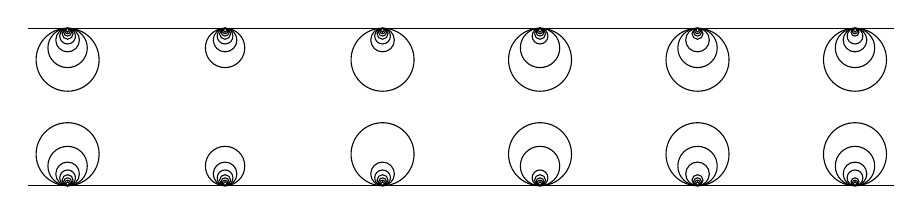
\begin{tikzpicture}
        \draw (-1.5,2) -- (9.5,2);
        \draw (-1.5,0) -- (9.5,0);

        \foreach \x in {0.8,0.5,0.3,0.2,0.14,0.1,0.07,0.05}
        {
            \draw (-1,2) arc (90:450:\x/2);
            \draw (-1,0) arc (270:630:\x/2);
        }
        
        \mydraw{1}{0}{0.8};

        \foreach \x in {0.5,0.3,0.2,0.14,0.1,0.07,0.05}
        {
            \draw (1,2) arc (90:450:\x/2);
            \draw (1,0) arc (270:630:\x/2);
        }

        \mydraw{3}{0}{0.5};

        \foreach \x in {0.8,0.3,0.2,0.14,0.1,0.07,0.05}
        {
            \draw (3,2) arc (90:450:\x/2);
            \draw (3,0) arc (270:630:\x/2);
        }

        \mydraw{5}{0}{0.3};

        \foreach \x in {0.8,0.5,0.2,0.14,0.1,0.07,0.05}
        {
            \draw (5,2) arc (90:450:\x/2);
            \draw (5,0) arc (270:630:\x/2);
        }

        \mydraw{7}{0}{0.2};

        \foreach \x in {0.8,0.5,0.3,0.14,0.1,0.07,0.05}
        {
            \draw (7,2) arc (90:450:\x/2);
            \draw (7,0) arc (270:630:\x/2);
        }

        \mydraw{9}{0}{0.14};

        \foreach \x in {0.8,0.5,0.3,0.2,0.1,0.07,0.05}
        {
            \draw (9,2) arc (90:450:\x/2);
            \draw (9,0) arc (270:630:\x/2);
        }
        
    \end{tikzpicture}
\end{center}

\plabel{9}%
Let $f:X\rightarrow S^1$ be the map.
Since $f^*(\pi_1(X))$ has to be a finite subgroup of $\mathbb{Z}$ and is therefore the trivial group, $f$ could be lifted to $\tilde{f}:X\rightarrow\mathbb{R}$.
Then $f$ is nullhomotopic since $\tilde{f}$ is.

\plabel{10}%
$2$-sheeted:
This amounts to find all graphs with $2$ vertices where each vertex has degree $4$.
They are
\begin{itemize}
    \item (1) on p.58,
    \item (1) on p.58 with $a$ and $b$ swapped, and
    \item (2) on p.58.
\end{itemize}
$3$-sheeted:
This amounts to find all graphs with $3$ vertices where each vertex has degree $4$.
They are
\begin{itemize}
    \item (3) on p.58,
    \item (5) on p.58,
    \item (6) on p.58,
    \item the following,
    \begin{center}
        \begin{tikzpicture}[decoration={
            markings,
            mark=at position 0.5 with {\arrow{latex}}}
            ]
            \draw[postaction={decorate}] (-30:1.5) to (90:1.5);
            \draw[postaction={decorate}] (90:1.5) to (210:1.5);
            \draw[postaction={decorate}] (210:1.5) to (-30:1.5);
            \draw[postaction={decorate}] (-30:1.5) arc (150:510:0.75);
            \draw[postaction={decorate}] (90:1.5) arc (-90:270:0.75);
            \draw[postaction={decorate}] (210:1.5) arc (30:390:0.75);
            \draw (30:1) node {$a$};
            \draw (150:1) node {$a$};
            \draw (270:1) node {$a$};
            \draw (-30:2.5) node {$b$};
            \draw (90:2.5) node {$b$};
            \draw (210:2.5) node {$b$};
        \end{tikzpicture}
    \end{center}
    \item the above with $a$ and $b$ swapped,
    \item the following, and
    \begin{center}
        \begin{tikzpicture}[decoration={
            markings,
            mark=at position 0.5 with {\arrow{latex}}}
            ]
            \draw[postaction={decorate}] (-30:1.5) to (90:1.5);
            \draw[postaction={decorate}] (90:1.5) to (210:1.5);
            \draw[postaction={decorate}] (210:1.5) to (-30:1.5);
            \draw[postaction={decorate}] (90:1.5) arc (-90:270:0.75);
            \draw (30:1) node {$a$};
            \draw (150:1) node {$a$};
            \draw (270:1) node {$a$};
            \draw (-90:0) node {$b$};
            \draw (90:2.5) node {$b$};
            \draw (-90:1.5) node {$b$};
            \draw[postaction={decorate}] (210:1.5) to[bend left] (-30:1.5);
            \draw[postaction={decorate}] (-30:1.5) to[bend left] (210:1.5);
        \end{tikzpicture}
    \end{center}
    \item the above with $a$ and $b$ swapped.
\end{itemize}


\plabel{12}%
The following covering is normal since for each the deck transformation acts transitively.
Since the generators of the fundamental group are mapped to $a^2$, $b^2$, and $(ab)^2$, the fundamental group is mapped to the normal subgroup generated by these elements.
\begin{center}
    \begin{tikzpicture}[decoration={
        markings,
        mark=at position 0.5 with {\arrow{latex}}}
        ]
        \draw[postaction={decorate}] (-22.5:2) to[bend left] (22.5:2);
        \draw[postaction={decorate}] (22.5:2) to[bend left] (67.5:2);
        \draw[postaction={decorate}] (67.5:2) to[bend left] (112.5:2);
        \draw[postaction={decorate}] (112.5:2) to[bend left] (157.5:2);
        \draw[postaction={decorate}] (157.5:2) to[bend left] (202.5:2);
        \draw[postaction={decorate}] (202.5:2) to[bend left] (247.5:2);
        \draw[postaction={decorate}] (247.5:2) to[bend left] (292.5:2);
        \draw[postaction={decorate}] (292.5:2) to[bend left] (337.5:2);
        \draw (0:2.25) node {$a$};
        \draw (45:2.25) node {$b$};
        \draw (90:2.25) node {$a$};
        \draw (135:2.25) node {$b$};
        \draw (180:2.25) node {$a$};
        \draw (225:2.25) node {$b$};
        \draw (270:2.25) node {$a$};
        \draw (315:2.25) node {$b$};
        \draw[postaction={decorate}] (22.5:2) to[bend left] (-22.5:2);
        \draw[postaction={decorate}] (67.5:2) to[bend left] (22.5:2);
        \draw[postaction={decorate}] (112.5:2) to[bend left] (67.5:2);
        \draw[postaction={decorate}] (157.5:2) to[bend left] (112.5:2);
        \draw[postaction={decorate}] (202.5:2) to[bend left] (157.5:2);
        \draw[postaction={decorate}] (247.5:2) to[bend left] (202.5:2);
        \draw[postaction={decorate}] (292.5:2) to[bend left] (247.5:2);
        \draw[postaction={decorate}] (337.5:2) to[bend left] (292.5:2);
        \draw (0:1.5) node {$a$};
        \draw (45:1.5) node {$b$};
        \draw (90:1.5) node {$a$};
        \draw (135:1.5) node {$b$};
        \draw (180:1.5) node {$a$};
        \draw (225:1.5) node {$b$};
        \draw (270:1.5) node {$a$};
        \draw (315:1.5) node {$b$};
    \end{tikzpicture}
\end{center}

\plabel{26(a)}%
If $\tilde{x}_0$ and $\tilde{x}'_0$ are both in $p^{-1}(x_0)$, then they are in the same components if and only if there exists a path from $\tilde{x}_0$ to $\tilde{x}'_0$, i.e. if and only if there is an element of $\pi_1(X)$ that send $\tilde{x}_0$ to $\tilde{x}'_0$.

\plabel{(b)}%

\prule

\plabel{2.1.11}%
That is, $i_\sharp(\sigma) - i_\sharp(\tau)$ is boundary implies $\sigma - \tau$ is a boundary.
It suffices to prove that $i_\sharp(\sigma)$ is boundary then $\sigma$ is boundary.
Let $\partial \sigma_Y = i_\sharp(\sigma)$.
Then $\partial (r_\sharp(\sigma_Y)) = r_\sharp (\partial\sigma_Y) = r_\sharp (i_\sharp (\sigma)) = \sigma$ since $ri = \operatorname{id}$.

\plabel{12}%
If
\[ \partial P + P \partial = g_\sharp - f_\sharp \]
and
\[ \partial Q + Q \partial = h_\sharp - g_\sharp \]
then
\[ \partial (P+Q) + (P+Q)\partial = h_\sharp - f_\sharp \]
and therefore the relation is transitive.
It's clear that the relation is reflective (by $P\rightarrow -P$) and symmetric ($P=0$).

\plabel{15}%
That is, $A\rightarrow B$ is surjective is equivalent to $A\rightarrow B \rightarrow 0$ is exact and $D\rightarrow E$ is injective is equivalent to $0\rightarrow D\rightarrow E$ is exact.
\begin{itemize}
    \item $A\xrightarrow{f} B$ is surjective $\Leftrightarrow$ $\operatorname{Im} f = B$ $\Leftrightarrow$ $A\rightarrow B \rightarrow 0$ is exact.
    \item $D\xrightarrow{g} E$ is injective $\Leftrightarrow$ $\operatorname{Ker} g = 0$ $\Leftrightarrow$ $0\rightarrow D\rightarrow E$ is exact.
\end{itemize}

\plabel{20}%
Since $CX$ is contractible,
\begin{align*}
    \tilde{H}_{n+1}(SX) &= \tilde{H}_{n+1}(CX/X) \\
    &= \tilde{H}_n(X).
\end{align*}
Let $Y_k$ denote the complex obtained by gluing $k$ copies of $CX$ along $X$.
Then
\begin{align*}
    \tilde{H}_{n+1}(Y_{k+1}) &= H_{n+1}(Y_k,X) \\
    &= \tilde{H}_{n+1}(Y_k/X) \\
    &= \tilde{H}_{n+1}(\vee^{k+1}SX) \\
    &= \oplus^{k+1} \tilde{H}_n(X).
\end{align*}

\plabel{22}%



\end{document}
